% This LaTeX was auto-generated from MATLAB code.
% To make changes, update the MATLAB code and export to LaTeX again.

\documentclass{article}

\usepackage[utf8]{inputenc}
\usepackage[T1]{fontenc}
\usepackage{lmodern}
\usepackage{graphicx}
\usepackage{color}
\usepackage{hyperref}
\usepackage{amsmath}
\usepackage{amsfonts}
\usepackage{epstopdf}
\usepackage[table]{xcolor}
\usepackage{matlab}

\sloppy
\epstopdfsetup{outdir=./}
\graphicspath{ {./fsk_images/} }

\begin{document}

\matlabtitle{Project Digital Communications  }

\begin{matlabcode}

clear all;
close all;
clc;

warning('off','all');
warning;
\end{matlabcode}
\begin{matlaboutput}
All warnings have the state 'off'.
\end{matlaboutput}
\begin{matlabcode}

\end{matlabcode}

\matlabheading{Message Signal Generation}

\begin{matlabcode}
Noit=1e4;
%Generate 1 and 0s
x = randi([0 1],Noit,1);   % Message signal in binary form 

figure(1);
subplot(2,2,1); 
stairs(x(1:8),'Linewidth',2);      %Message signal plot 
title('Message signal'); 
ylabel('Amplitude'); 

\end{matlabcode}

\matlabheading{Carrier Signal Generation}


\vspace{1em}
\begin{matlabcode}
Tb = 0.002;      % symbol duration in sec
br = 1/Tb;       % Bit rate

fs = 1000;       % Sampling Frequency

fc0 = 3000;      % Carrier frequency for binary input '0'
fc1 = fc0 + br;  % Carrier frequency for binary input '1'

%time window, the duration between two samples is 1/(100*fs)
t1=0:1/(100*fs):Tb;

%Signal Generation Carrier Waveform
s1 = cos(2*pi*fc0*t1);
s2 = cos(2*pi*fc1*t1);

% Signal Generation for Quadrature Implementation
s3 = sin(2*pi*fc0*t1);
s4 = sin(2*pi*fc1*t1);

% Carrier Signal Plot
subplot(2,2,2); 
plot(t1,s1);
title('Carrier Signal Fc0 3Khz'); 
xlabel('Time'); 
ylabel('Amplitude'); 

subplot(2,2,3); 
plot(t1,s2);
title('Carrier Signal Fc1 3.5 Khz'); 
xlabel('Time'); 
ylabel('Amplitude'); 

\end{matlabcode}

\matlabheading{Signal Modulation}


\vspace{1em}
\begin{matlabcode}
mod_Signal = [];
for (i = 1:1:Noit)
    if (x(i) == 1)
        y = cos(2*pi*fc0*t1);   % Modulation signal with carrier signal 1
    else
        y = cos(2*pi*fc1*t1);   % Modulation signal with carrier signal 2
    end
    mod_Signal = [mod_Signal y];
end

% Total Signal Duration
t2 = 0:1/(100*fs):Tb*Noit;

\end{matlabcode}

\matlabheading{Modulated Signal Plot}

\begin{matlabcode}
subplot(2,2,4); 
plot(t2(1:8*length(t1)),mod_Signal(1:8*length(t1)));
title('Modulated Signal for 8 bits'); 
xlabel('Time'); 
ylabel('Amplitude');
\end{matlabcode}
\begin{center}
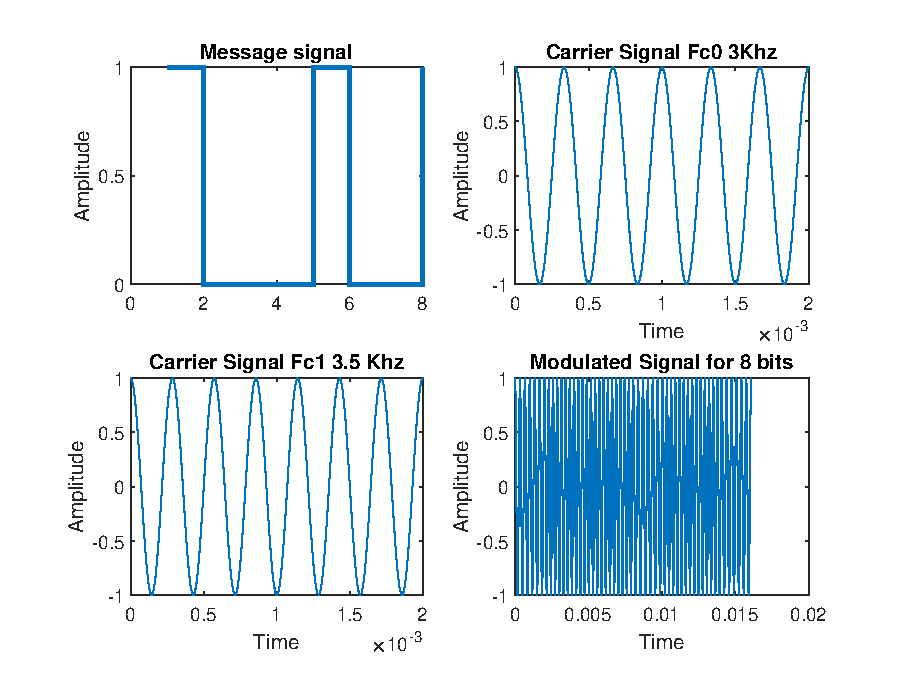
\includegraphics[width=\maxwidth{56.196688409433015em}]{figure_0.eps}
\end{center}
\begin{matlabcode}

\end{matlabcode}

\matlabheading{Recieved Signal Generation}

\begin{matlabcode}
 
rx_Signal = [];

\end{matlabcode}

\begin{par}
\begin{flushleft}
AWGN Addition
\end{flushleft}
\end{par}

\matlabheading{Modulated Signals vs Signal with AWGN (8 Bits) }

\begin{matlabcode}
step1 = length(mod_Signal)/11;
snrdB = -10;
for n1 = step1:step1:length(mod_Signal) %define SNR in terms of dB
    rx_Signal = [rx_Signal awgn(mod_Signal(n1-(step1-1):n1),snrdB)];
    snrdB = snrdB + 2;
end



figure(2);
subplot(2,1,1); 
plot(t2(1:8*length(t1)),mod_Signal(1:8*length(t1)));      %Modulated Signal Plot 
title('Modulated signal'); 
ylabel('Amplitude'); 
    
subplot(2,1,2); 
plot(t2(1:8*length(t1)),rx_Signal(1:8*length(t1)));      %RX Signal Plot with Noise
title('RX signal with AWGN'); 
ylabel('Amplitude'); 
\end{matlabcode}
\begin{center}
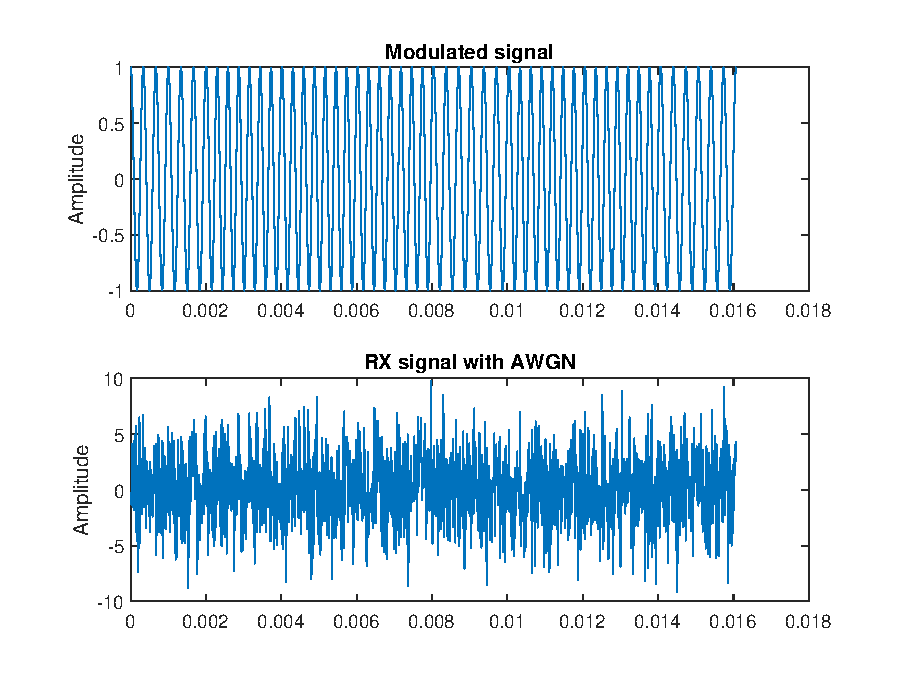
\includegraphics[width=\maxwidth{56.196688409433015em}]{figure_1.eps}
\end{center}
\begin{matlabcode}

\end{matlabcode}

\matlabheading{FSK Demodulation}

\begin{matlabcode}
 

s = length(t1);

step = rx_Signal / s;

demod = [];
demod2 = [];

\end{matlabcode}

\matlabheading{Correlation}

\begin{matlabcode}

for n = s:s:length(rx_Signal)
  
\end{matlabcode}

\vspace{1em}

\begin{matlabcode}
  cor1 = corrcoef(sqrt(2/Tb).*s1,rx_Signal(n-(s-1):n));    
  cor2 = corrcoef(sqrt(2/Tb).*s2,rx_Signal(n-(s-1):n));
  cor3 = corrcoef(sqrt(2/Tb).*s3,rx_Signal(n-(s-1):n));
  cor4 = corrcoef(sqrt(2/Tb).*s4,rx_Signal(n-(s-1):n));
  
 
\end{matlabcode}

\matlabheadingtwo{Squaring and IQ EnergySummation}

\begin{matlabcode}
 
  IQ1 = cor1.^2 + cor3.^2;
  IQ2 = cor2.^2 + cor4.^2;
  
  IQ = IQ1-IQ2;
  
  
\end{matlabcode}

\matlabheadingtwo{Test Statistics and Decision}

\begin{matlabcode}
  if(IQ(2) > 0);
      a = 1;
  else;
     a = 0;
  end   
  
  demod2 = [demod2 a];

end

demod2 = transpose(demod2);

BER_theory=[];
BER_sim=[];

step1 = length(demod2)/11;
i1 = 1;
i2 = step1;

\end{matlabcode}

\matlabheading{Error Probabilty}

\begin{matlabcode}
for (snrdB=-10:2:10) %define SNR in terms of dB
    BER_theory = [BER_theory berawgn(snrdB,'fsk',2,'noncoherent')];
    BER_sim = [BER_sim biterr(x(i1:i2),demod2(i1:i2))];
    i1 = i2 + 1;
    i2 = i2 + step1;
end

\end{matlabcode}

\matlabheading{\textbf{SNR vs Probabilty of Error Plot}}

\begin{matlabcode}
figure(3);
semilogy((-10:2:10), BER_theory);
hold on;
semilogy((-10:2:10), BER_sim);
ylabel('Probability of bit error');
xlabel('Eb/No (dB)')
grid on;
\end{matlabcode}
\begin{center}
\includegraphics[width=\maxwidth{56.196688409433015em}]{figure_2.eps}
\end{center}
\begin{matlabcode}


\end{matlabcode}

\matlabheading{Recovered Signal Plot}

\begin{matlabcode}
figure(4);
subplot(2,1,1); 
stairs(x(1:100),'Linewidth',2);      %Message signal plot 
title('Message signal'); 
ylabel('Amplitude'); 

subplot(2,1,2); 
stairs(demod2(1:100),'Linewidth',2);      %Message signal plot 
title('Demodulated'); 
ylabel('Amplitude'); 
\end{matlabcode}
\begin{center}
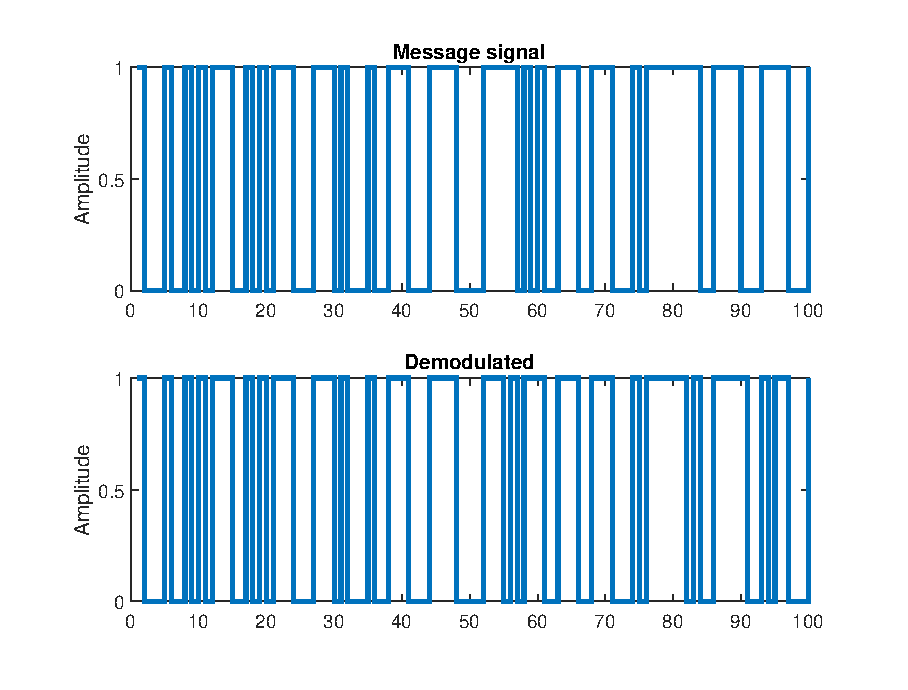
\includegraphics[width=\maxwidth{56.196688409433015em}]{figure_3.eps}
\end{center}
\begin{matlabcode}


\end{matlabcode}

\end{document}
